% LaTeX Article Template - customizing header and footer
\documentclass{article}

\newtheorem{thm}{Theorem}

% Set left margin - The default is 1 inch, so the following
% command sets a 1.25-inch left margin.
\setlength{\oddsidemargin}{0.25in}

% Set width of the text - What is left will be the right margin.
% In this case, right margin is 8.5in - 1.25in - 6in = 1.25in.
\setlength{\textwidth}{6in}

% Set top margin - The default is 1 inch, so the following
% command sets a 0.75-inch top margin.
\setlength{\topmargin}{-0.25in}

% Set height of the header
\setlength{\headheight}{0.1in}

% Set vertical distance between the header and the text
\setlength{\headsep}{0.2in}

% Set height of the text
\setlength{\textheight}{9in}

% Set vertical distance between the text and the
% bottom of footer
%\setlength{\footskip}{0.15in}

% Set the beginning of a LaTeX document
\usepackage{multirow}
\usepackage{fullpage}
\usepackage{graphicx}
\usepackage{amsthm}
\usepackage{amssymb}
\usepackage{amssymb}
\usepackage{algpseudocode}
\usepackage{caption}
\usepackage{float}
\usepackage{subcaption}
\graphicspath{%
    {converted_graphics/}% inserted by PCTeX
    {/}% inserted by PCTeX
}
%%%%%%%%%%%%%%%%%%%%%%%%%%%%%

\begin{document}\title{Chaos Game Analysis\\ Spring 2017\\ Math-M330}         % Enter your title between curly braces
\author{Steven Myers}        % Enter your name between curly braces
\date{\today}          % Enter your date or \today between curly braces
\maketitle


% Redefine "plain" pagestyle
\makeatother     % `@' is restored as a "non-letter" character

% Set to use the "plain" pagestyle
\pagestyle{plain}

\section*{Introduction to the Chaos Game}

\paragraph{}
The chaos game is an iterative process that will produce an image known as the Sierpinski triangle. Images like the Sierpinski triangle are called\textit{fractals}. A fractal is an image that is created by an iterable, mathematical process. Fractals have unique mathematical qualities that can be discovered by observation. We will explore the unique qualities of the Sierpinski triangle by observing its formation from the chaos game. The rules for how to play the chaos game are listed below for reference:
\begin{enumerate}
    \item
    Start by placing three points on a piece of paper. For the best results, try placing the points roughly in the three vertices of an equilateral triangle.
    \item
    Next, select an initial point contained within the area of the vertices, or above of the invisible edges connecting the three vertices you drew.
    \item
    Select one of the three points of the triangle randomly. (You may use a dice or random number generator)
    \item
    Draw a new point halfway between the randomly selected vertex and your initial starting point.
    \item
    Repeat step 3 until a pattern emerges or until satisfied.
\end{enumerate}
\paragraph{}
In the first iterations of the chaos game, it's likely that the generated points fall along defined edges at different angles leading towards the three vertices. This early pattern that one may notice is that the points will follow a "tug-of-war" pattern, moving back and forth between just two the vertices and forming what appears to be a defined edge. You may even begin to notice an upside down triangle circumscribed within our original area between the three vertices. Using a computer program, we can generate more points than what would be possible by pencil and paper. In Figure 1, we can view a few resulting images of the chaos game, generated by a computer program.
\begin{figure}[H]
    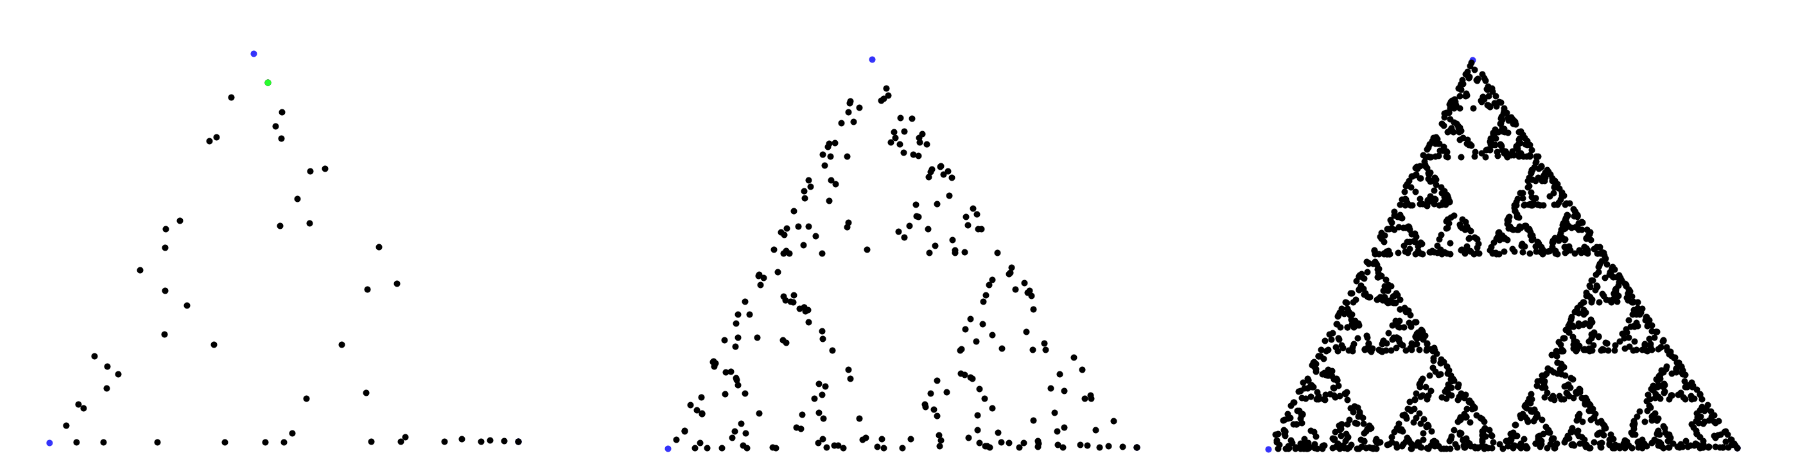
\includegraphics[width=\linewidth, height=.2\textheight]{combined_image}
    \caption{Images created by the Chaos Game for 50, 250, and 1000 iterations respectively.}
\end{figure}
\begin{figure}[H]
    \centering
    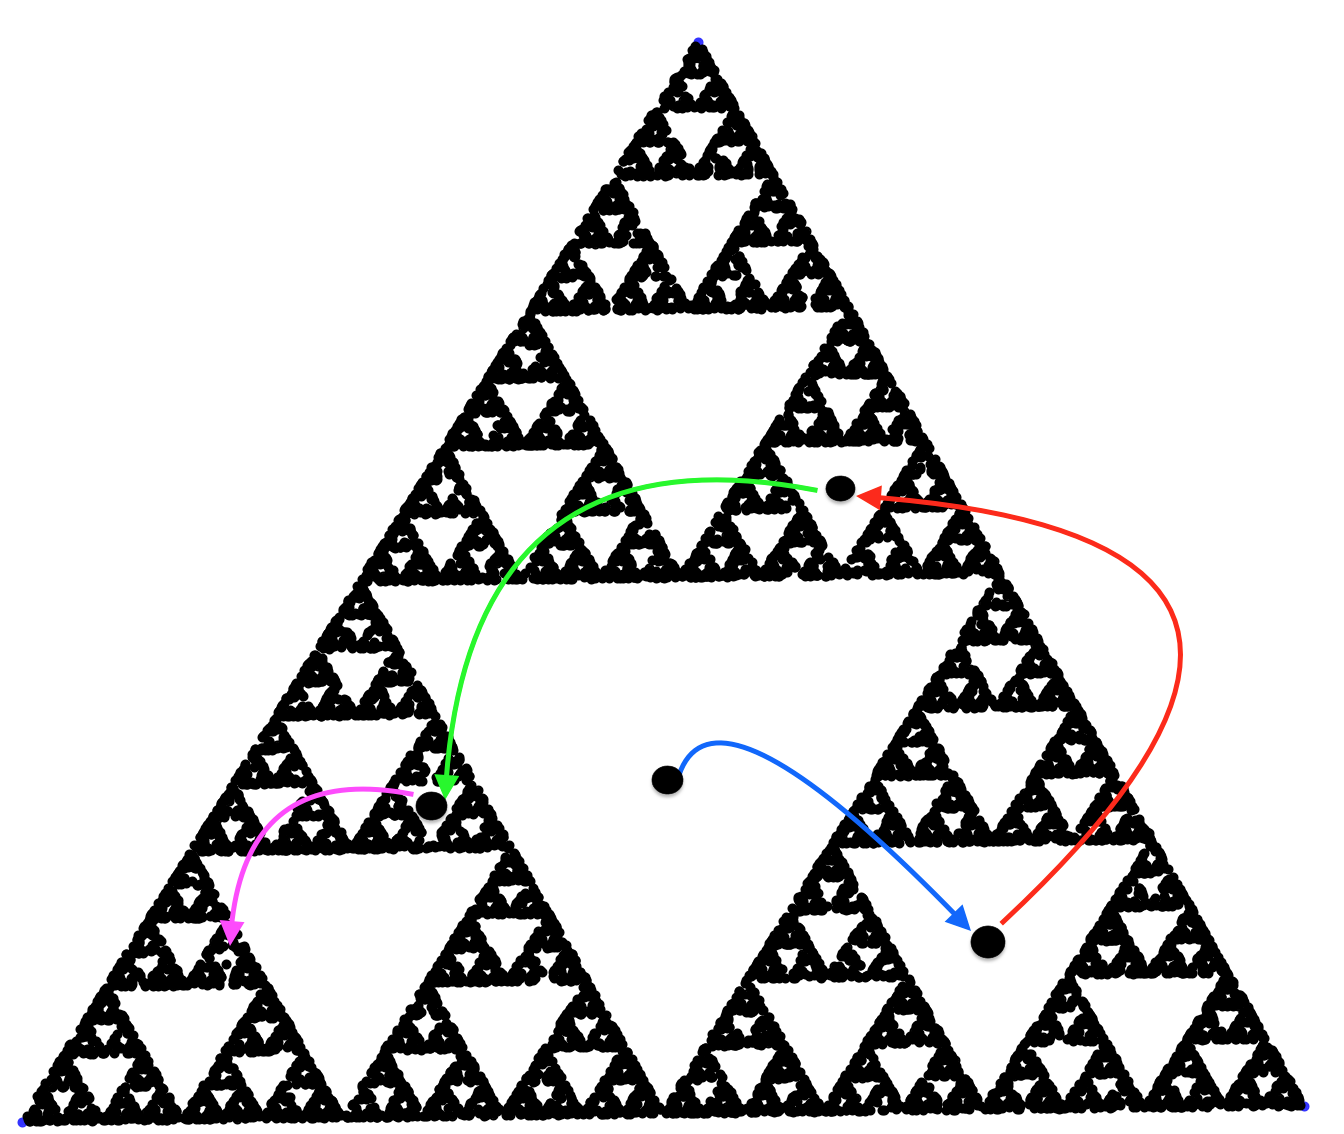
\includegraphics[width=.5\linewidth, height=.25\textheight]{centered_start}
    \caption{Initial starting point in the center of the original triangle. Centered points have been enlarged for clarity and colored arrows show the iterations of the chaos game.}
\end{figure}
\paragraph{}
Looking at Figure 1, we can immediately see that there are well-defined spaces where no points fall. When we iterate 250 times or more, we begin to see these spaces fully develop as upside down, circumscribed triangles. If we try replay the chaos game by hand and select new initial starting points, we will find that no initial starting point can produce subsequent points within these zones where no points fall, no matter the initial starting point we choose \textit{except} if we choose an initial starting point that is directly within one of the upside down triangles where no points fall. However, even when we purposefully select an initial starting point in zones where no points fall, we will still eventually get the same image as other initial starting points. Moreover, we will not produce points that are \textit{closer} to the center than our initial point. An example of this phenomenon is found in Figure 2.
\paragraph{}
 So, by iteratively working the chaos game out, we see that a common pattern emerges that is \textit{not} random. We have consistent areas in which no points fall, and we eventually get the same resulting image regardless of our initial starting point.
\section*{The Sierpinski Triangle}
\begin{figure}[H]
    \centering
    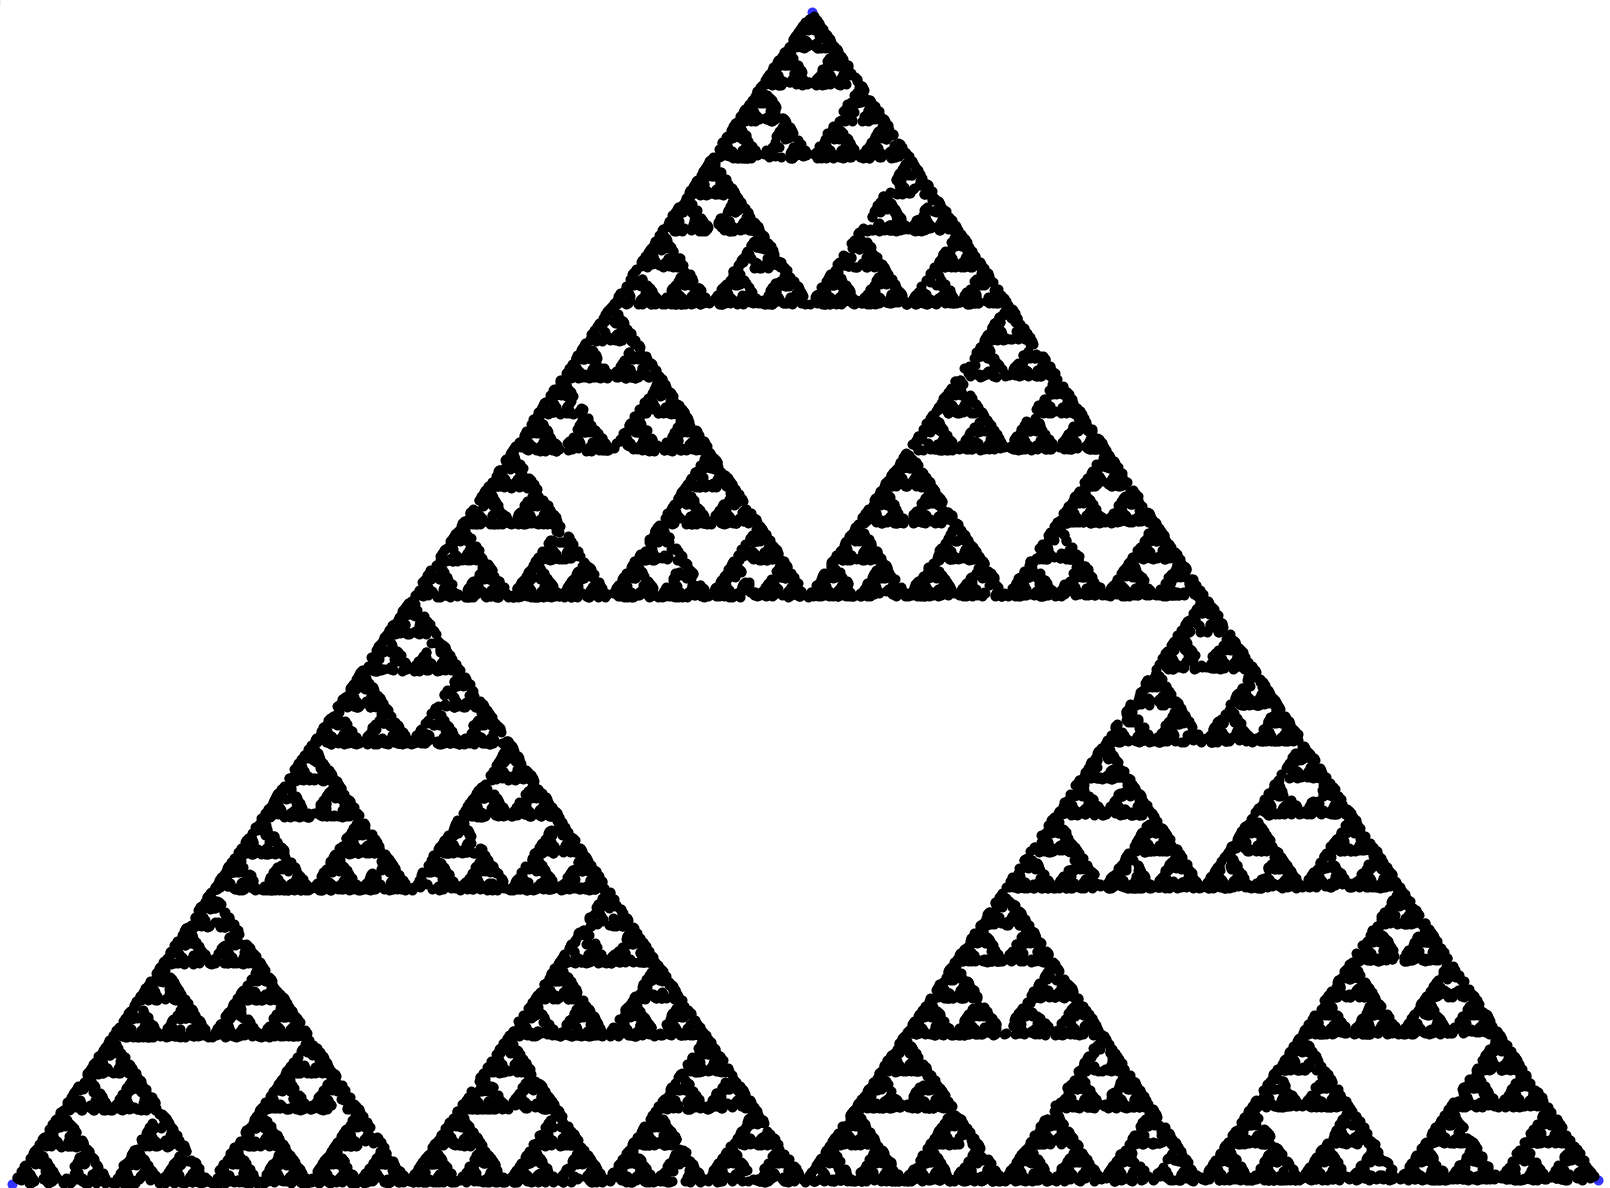
\includegraphics[width=.5\linewidth, height=.25\textheight]{ideal}
    \caption{The ideal Sierpinski triangle shape.}
\end{figure}
\paragraph{}
When the chaos game is iterated infinitely many times, it eventually produces the Sierpinski triangle. In an ideal Sierpinski triangle, all of the edges are fully formed as we can nearly see in the later iterations of the chaos game. Figure 3 shows the fully formed Sierpinski triangle. The Sierpinski triangle has a number of unique qualities that extend beyond how the points fall in the chaos game. It consists of smaller Sierpinski triangles in its three sub-triangles. Subtriangles are formed by the circumscribed upside triangles in the center of each Sierpinski triangle - forming four triangles of \(\frac{1}{4}\) the surface area of the original triangle. The upside triangle in the center serves as "lost space" where the image is no longer created. We can think of this as lost surface area.
\paragraph{}
Like we did with the chaos game, we can come up with a series of steps to create the ideal Sierpinski triangle shape:
\begin{enumerate}
    \item Draw an equilateral triangle.
    \item Draw an upside down equilateral triangle within the equilateral triangle. This triangle should be \(\frac{1}{4}\) of the size of the original, and its vertices will be the midpoints of the edges of the original triangle.
    \item Repeat step 2 indefinitely for the three upright, smaller subtriangles.
\end{enumerate}
\paragraph{}
With this new set of instructions, we can begin to make further observations about the Sierpinski triangle. We can immediately notice that every time we create a new Sierpinski triangle, the original triangle loses a quarter of its surface area. The surface area is \textit{lost} in the sense that no further iterations of the Sierpinski triangle are generated in the upside down triangles. In terms of the chaos game, the surface area is lost since no points will ever fall within the the middle of the triangle. Since the ideal Sierpinski triangle shape continues indefinitely within its subtriangles, and we know that from each iteration a quarter of surface area is lost, we can deduce that the area of our original Sierpinski triangle approachs a limit of zero surface area. So, we have a shape that essentially has zero surface area.
\paragraph{}
Another interesting quality of the ideal Sierpinksi triangle is the length of all of its edges. In each iteration of the triangle, the side length of an interior iteration is exactly half the side length of the previous triangle. Three new line segments (the edges of the upside down, circumscribed triangle) are formed in every iteration. That means that in every iteration of the fractal, the total length of all the line segments in the triangle increases by 3/2. If we iterate to infinity, we will also notice that the sum of all the line segments approaches infinity. So, the Sierpinksi triangle has a surface area that approaches zero, while its perimeter approaches infinity.
\paragraph{}
If the ideal Sierpinski triangle has \textit{zero} surface area, or at least an infinitesimally small surface area, then we must consider whether or not the Sierpinski triangle is actually a 2D shape since a property of 2D shapes is its surface area. We know that 1D shapes are comprised completely of a single line segment and 2D shapes consist of many line segments. Since the Sierpinksi triangle has more than one line segment, we can definitively say it's not a 1D shape. However, since its surface area approaches zero, it also is not necessarily a two dimensional shape.
\section*{Dimensionality}
\paragraph{}
The Hausdorff-Besicovitch dimension is a way of representing the dimensionality of shapes, and it allows us to quantify the dimensionality of fractal shapes, namely the Sierpinksi triangle in our scenario. The formula for calculating dimensionality. \(D\) is given by:
\[D = \frac{\log(N)}{\log(r)} \]
where \(N\) is the expansion factor of a fractal shape, and \(r\) is the scaling factor of the repeated shape. We know that the Sierpinksi triangle generates three new Sierpinkski triangles in every iteration, so \(N=3\). We also know that the side length of the new triangles that are formed are exactly half the length of the previous iteration's side length, so \(r=2\). Putting it all together, we can solve for the Sierpinksi triangle's dimension:
\[D = \frac{\log(N)}{\log(r)} = \frac{\log(3)}{\log(2)} \approx 1.585\]
\paragraph{}
In conclusion, the Sierpinkski triangle is a mathematically interesting shape generated by self replicating cycles. Its dimensionality is between 1D and 2D due to the nature of its surface area while still existing in 2D space. Under further examination, the Sierpinksi triangle could yield interesting properties when given a 3D form as a tetrahedron.

\medskip

\begin{thebibliography}{9}
\bibitem{wikipedia1}
Wikipedia contributors. "Sierpinski triangle." Wikipedia, \textit{The Free Encyclopedia}. Wikipedia, The Free Encyclopedia, 14 Feb. 2017. Web. 24 Feb. 2017.

\bibitem{wikipedia2}
Wikipedia contributors. "Hausdorff dimension." Wikipedia, \textit{The Free Encyclopedia.} Wikipedia, The Free Encyclopedia, 10 Jan. 2017. Web. 24 Feb. 2017.

\bibitem{online_site}
"Fractal Dimension." \textit{Fractal Foundation Online Course - Chapter 1 - FRACTALS IN NATURE.} N.p., n.d. Web. 24 Feb. 2017.
\end{thebibliography}
\end{document}
